\documentclass{standalone}
\usepackage{tikz}
\begin{document}
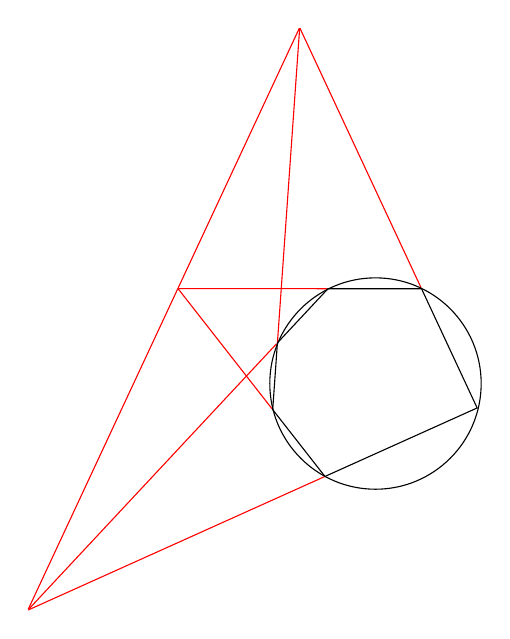
\begin{tikzpicture}[x=1pt,y=1pt]
\draw[red] (129.94,-127.19) -- (76.20,-127.18);
\draw[red] (111.67,-147.09) -- (22.24,-242.86);
\draw[red] (163.89,-126.87) -- (120.13,-33.09);
\draw (147.41,-161.46) circle (38.19);
\draw[red] (21.93,-243.29) -- (129.06,-195.07);
\draw[red] (120.01,-33.07) -- (111.99,-146.51);
\draw[red] (76.13,-127.25) -- (110.01,-170.56);
\draw (164.05,-127.20) -- (130.24,-127.20) -- (111.97,-146.76) -- (110.27,-170.89) -- (129.15,-195.03) -- (184.15,-170.28) -- cycle;
\draw[red] (119.87,-33.12) -- (21.97,-242.94);
\end{tikzpicture}
\end{document}
